\documentclass{article}
\usepackage[T1]{fontenc}
\usepackage{lmodern}
\usepackage{graphicx}
\usepackage{amsmath,amssymb}
\usepackage[a4paper,margin=2cm]{geometry}
\usepackage[absolute,overlay]{textpos}
\setlength{\TPHorizModule}{1mm}
\setlength{\TPVertModule}{1mm}
\usepackage[indonesian]{babel}
\usepackage{hyperref}
\setlength{\emergencystretch}{2em}
% unit: Halaman 51

\begin{document}

% === Halaman 51 (llm) ===

\vspace{103.95mm}

\begin{verbatim}
# Program utama (pemanggilan fungsi enkripsi dan dekripsi AES)
file_plaintext = input("Ketikkan nama file input pesan yang akan dienkripsi: (beserta path) ")
file_ciphertext = input("Ketikkan nama file output pesan hasil enkripsi (beserta path): ")
kunci = input("Kunci?:")
encrypt_file(file_plaintext, file_ciphertext, kunci)
print("Enkripsi selesai. Hasil disimpan di:", file_ciphertext)

file_ciphertext = input("Ketikkan nama file input pesan yang akan didekripsi: (beserta path) ")
file_plaintext = input("Ketikkan nama file output pesan hasil dekripsi (beserta path): ")
kunci = input("Kunci?:")
decrypt_file(file_ciphertext, file_plaintext, kunci)
print("Dekripsi selesai. Hasil disimpan di:", file_plaintext)
\end{verbatim}

% deskripsi: Potongan kode Python untuk implementasi program utama enkripsi dan dekripsi AES
% bbox normalisasi: [0.0400, 0.1900, 0.8800, 0.5400]
\begin{textblock*}{176.40mm}(8.40mm,56.43mm)
\noindent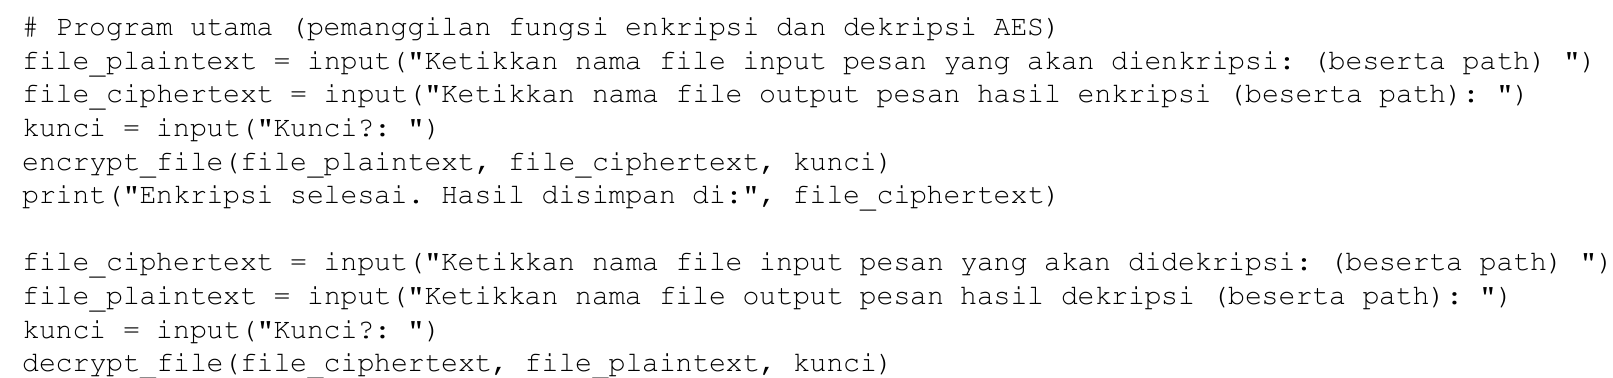
\includegraphics[width=176.40mm,height=103.95mm]{../../images/llm/page_051_img_01.png}%
\end{textblock*}

\end{document}
